\section{eo\-Seq\-Populator$<$ EOT $>$ Class Template Reference}
\label{classeo_seq_populator}\index{eoSeqPopulator@{eoSeqPopulator}}
Seq\-Populator: an {\bf eo\-Populator}{\rm (p.\,\pageref{classeo_populator})} that sequentially goes through the population is supposed to be used after a batch select of a whole bunch or genitors.  


{\tt \#include $<$eo\-Populator.h$>$}

Inheritance diagram for eo\-Seq\-Populator$<$ EOT $>$::\begin{figure}[H]
\begin{center}
\leavevmode
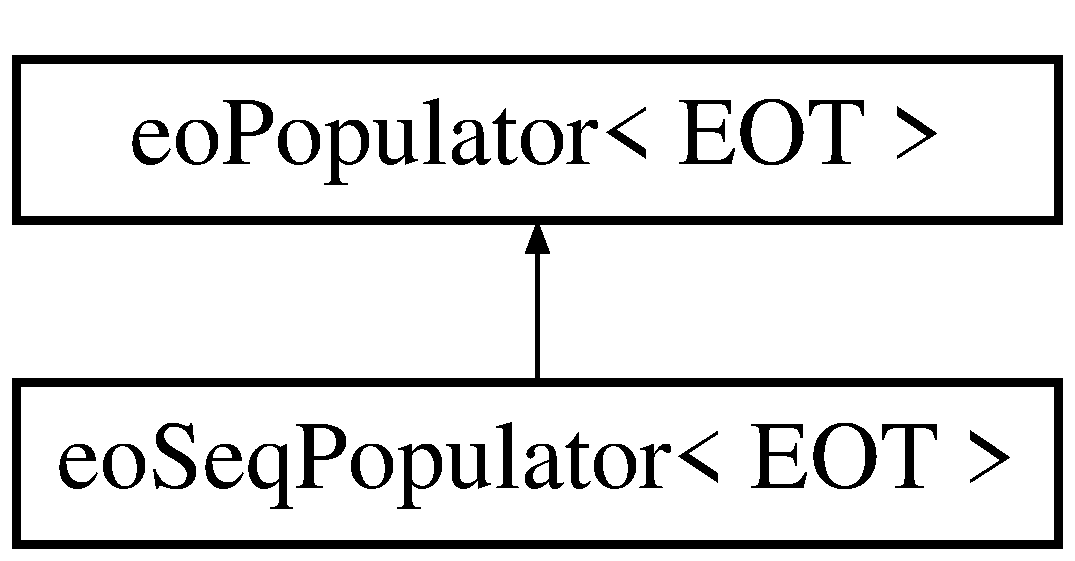
\includegraphics[height=2cm]{classeo_seq_populator}
\end{center}
\end{figure}
\subsection*{Public Member Functions}
\begin{CompactItemize}
\item 
{\bf eo\-Seq\-Populator} (const {\bf eo\-Pop}$<$ {\bf EOT} $>$ \&\_\-pop, {\bf eo\-Pop}$<$ {\bf EOT} $>$ \&\_\-dest)\label{classeo_seq_populator_a0}

\item 
const {\bf EOT} \& {\bf select} (void)\label{classeo_seq_populator_a1}

\begin{CompactList}\small\item\em the select method simply returns next individual in the src pop \item\end{CompactList}\end{CompactItemize}
\subsection*{Private Attributes}
\begin{CompactItemize}
\item 
unsigned {\bf current}\label{classeo_seq_populator_r0}

\end{CompactItemize}


\subsection{Detailed Description}
\subsubsection*{template$<$class EOT$>$ class eo\-Seq\-Populator$<$ EOT $>$}

Seq\-Populator: an {\bf eo\-Populator}{\rm (p.\,\pageref{classeo_populator})} that sequentially goes through the population is supposed to be used after a batch select of a whole bunch or genitors. 



Definition at line 152 of file eo\-Populator.h.

The documentation for this class was generated from the following file:\begin{CompactItemize}
\item 
eo\-Populator.h\end{CompactItemize}
